\section{Optimierung der Empfehlungsqualität}
% V-Ansatz Teil 3 – Evaluation und Optimierung

\subsection{Zielfunktion und Evaluationsmetriken}
% Begrenzte Zusatzmetriken (Diversity, Serendipity)


\[
score_{ges} = w_{cbf} \cdot score_{cbf} + w_{cf} \cdot score_{cf}
\]

\subsection{Modellvarianten}
% CBF-Modell
% CF-Modell (z. B. LightFM, ALS)
% Hybridmodell (Score-Fusion: $\alpha \cdot \text{CBF} + (1 - \alpha) \cdot \text{CF}$)

\subsection{Optimierungsstrategie}
% α-Tuning (Score Fusion)
% Vergleichsbaselines
% Evaluation mit GA4-Daten
% content/figures/plot_hyperparameterraum.tex

\begin{figure}[H]
    \centering
    \includegraphics[width=0.9\textwidth]{content/figures/svg/hyperparameterraum.pdf}
    \caption{Visualisierung des zweidimensionalen Hyperparameterraums der Modellgewichtungen. Die Achsen repräsentieren die Gewichte für das CBF-Modell (\(w_{cbf}\)) und das CF-Modell (\(w_{cf}\)). Die Einfärbung der Punkte visualisiert den resultierenden NDCG@10-Wert für jede Konfiguration aus dem Optuna-Suchlauf.}
    \label{fig:hyperparameterraum}
\end{figure}

\subsection{Ergebnisse}
% % Tabellen: Precision@5, APS je α
% % Inhalt von: content/tables/vergleich_baselines.tex

\begin{table}[htbp]
    \centering
    \caption{Vergleich des optimierten Hybrid-Modells mit den Baseline-Modellen anhand der Metriken NDCG@10 und Hit Rate@10.}
    \label{tab:baseline_vergleich}
    \begin{tabular}{lrr}
        \toprule
        \textbf{Modell} & \textbf{NDCG@10} & \textbf{Hit Rate@10} \\
        \midrule
        Hybrid-Modell & 1.25\% & 1.8\% \\
        Popularity-Baseline        & 0.23\% & 0.6\% \\
        Recency-Baseline           & 0.14\% & 0.4\% \\
        \bottomrule
    \end{tabular}
\end{table}
% % Visualisierungen: Liniendiagramme, ggf. UMAP-Spaces
% % content/tables/statistiken_testdaten.tex

\begin{table}[htbp]
    \centering
    \caption{Statistische Kennzahlen des Test- und Validierungsdatensatzes, basierend auf den Klick-Logs der letzten Januarwoche.}
    \label{tab:statistiken_test}
    \begin{tabular}{lr}
        \toprule
        \textbf{Metrik} & \textbf{Wert} \\
        \midrule
        Gesamte Artikelaufrufe & 3.627.024 \\
        Einzigartige user\_pseudo\_ids & 1.099.289 \\
        Einzigartige Artikel & 57.100 \\
        \bottomrule
    \end{tabular}
\end{table}
% % content/tables/statistiken_trainingsdaten.tex

\begin{table}[H]
    \centering
    \caption{Statistische Kennzahlen des Trainingsdatensatzes, basierend auf den Klick-Logs der ersten drei Januarwochen.}
    \label{tab:statistiken_training}
    \begin{tabular}{lr}
        \toprule
        \textbf{Metrik} & \textbf{Wert} \\
        \midrule
        Gesamte Interaktionen (Klicks) & 11.412.116 \\
        Einzigartige user\_pseudo\_ids & 2.294.733 \\
        Einzigartige Artikel & 104.462 \\
        \bottomrule
    \end{tabular}
\end{table}
% % content/figures/plot_nutzerverteilung_test.tex

\begin{figure}[H]
    \centering
    \includegraphics[width=0.9\textwidth]{content/figures/svg/nutzer_verteilung_test.pdf}
    \caption{Verteilung der Nutzeraktivität im Testdatensatz. Die Verteilung ist analog zum Trainingsdatensatz und zeigt ebenfalls eine ausgeprägte Long-Tail-Struktur, was die Repräsentativität des Test-Splits unterstreicht.}
    \label{fig:nutzerverteilung_test}
\end{figure}
% % content/figures/plot_nutzerverteilung_train.tex

\begin{figure}[htbp]
    \centering
    \includegraphics[width=0.9\textwidth]{content/figures/svg/nutzer_verteilung_train.pdf}
    \caption{Verteilung der Nutzeraktivität im Trainingsdatensatz. Die Darstellung verdeutlicht die typische Long-Tail-Verteilung: Eine große Anzahl von Nutzern interagiert nur selten mit Artikeln, während eine kleine Gruppe von "Power-Nutzern" für einen Großteil der Klicks verantwortlich ist.}
    \label{fig:nutzerverteilung_train}
\end{figure}
% % content/figures/plot_artikelverteilung_test.tex

\begin{figure}[htbp]
    \centering
    \includegraphics[width=0.9\textwidth]{content/figures/svg/artikel_verteilung_test.pdf}
    \caption{Popularitätsverteilung der Artikel im Testdatensatz. Die charakteristische Long-Tail-Verteilung bleibt auch in der letzten Januarwoche bestehen, was auf eine stabile Grundstruktur des Nutzerinteresses hindeutet.}
    \label{fig:artikelverteilung_test}
\end{figure}
% % content/figures/plot_artikelverteilung_train.tex

\begin{figure}[H]
    \centering
    \includegraphics[width=0.9\textwidth]{content/figures/svg/artikel_verteilung_train.pdf}
    \caption{Popularitätsverteilung der Artikel im Trainingsdatensatz. Die Grafik zeigt, dass eine geringe Anzahl von Artikeln einen Großteil der Klicks auf sich vereint, während die Mehrheit der Artikel nur wenige Interaktionen erhält (Long-Tail).}
    \label{fig:artikelverteilung_train}
\end{figure}
% \subsection{Interpretation und Analyse}
% % Hybridisierung wirkungsvoll?
% % Trade-offs und Nutzenklärung
% % Ablationsidee: z. B. Ausschalten von CBF-/CF-Signal
% % content/figures/plot_2d_performance.tex

\begin{figure}[htbp]
    \centering
    \includegraphics[width=0.9\textwidth]{content/figures/svg/2d_performance.pdf}
    \caption{2D-Darstellung des Hyperparameterraums. Die Achsen zeigen die Gewichtungen für das CBF- (\(w_{cbf}\)) und CF-Modell (\(w_{cf}\)). Die Farbe der Punkte indiziert den erreichten NDCG@10-Score. Der optimale Punkt ist markiert.}
    \label{fig:2d_performance}
\end{figure}
% % content/figures/plot_3d_scatter.tex

\begin{figure}[htbp]
    \centering
    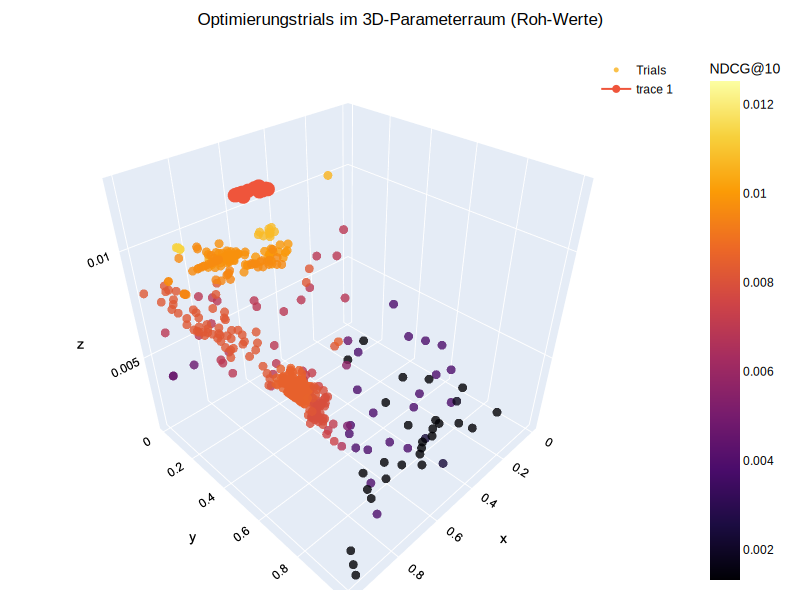
\includegraphics[width=0.8\textwidth]{content/figures/svg/3d_scatter_plot.pdf}
    \caption{Interaktives 3D-Streudiagramm der Optuna-Trials zur Visualisierung der Parameterabhängigkeiten. (Hinweis: Die Darstellung in der PDF-Version der Arbeit ist eine statische Ansicht).}
    \label{fig:3d_scatter}
\end{figure}
% % content/figures/plot_kontour.tex

\begin{figure}[H]
    \centering
    \includegraphics[width=0.9\textwidth]{content/figures/svg/kontourplot.pdf}
    \caption{Konturplot zur Darstellung der NDCG@10-Verteilung im zweidimensionalen Parameterraum der Modellgewichtungen. Die Isolinien verbinden Bereiche mit ähnlicher Performance.}
    \label{fig:kontourplot}
\end{figure}
% % content/figures/plot_optimierungsverlauf.tex

\begin{figure}[htbp]
    \centering
    \includegraphics[width=0.9\textwidth]{content/figures/svg/optimierungsverlauf.pdf}
    \caption{Visualisierung des Optimierungsverlaufs der 515 Optuna-Trials. Jeder Punkt stellt die NDCG@10-Metrik (Y-Achse) für einen bestimmten Trial (X-Achse) dar. Der Verlauf zeigt die Konvergenz des Optimierers gegen bessere Werte.}
    \label{fig:optimierungsverlauf}
\end{figure}
% % content/figures/plot_hyperparameterraum.tex

\begin{figure}[H]
    \centering
    \includegraphics[width=0.9\textwidth]{content/figures/svg/hyperparameterraum.pdf}
    \caption{Visualisierung des zweidimensionalen Hyperparameterraums der Modellgewichtungen. Die Achsen repräsentieren die Gewichte für das CBF-Modell (\(w_{cbf}\)) und das CF-Modell (\(w_{cf}\)). Die Einfärbung der Punkte visualisiert den resultierenden NDCG@10-Wert für jede Konfiguration aus dem Optuna-Suchlauf.}
    \label{fig:hyperparameterraum}
\end{figure}